%        File: report.tex
%     Created: Thu May 04 03:00 PM 2017 A
% Last Change: Thu May 04 03:00 PM 2017 A
%
\documentclass[conference, a4paper]{IEEEtran}

\usepackage{cite, graphicx, amsmath} 
\interdisplaylinepenalty=2500

% *** Do not adjust lengths that control margins, column widths, etc. ***
% *** Do not use packages that alter fonts (such as pslatex).         ***
% There should be no need to do such things with IEEEtran.cls V1.6 and later.


% correct bad hyphenation here
%\hyphenation{<+op-tical net-works semi-conduc-tor+>}


\begin{document}
%
% paper title
\title{Conceptual Design of a Real-Time Pedicle Screw Positioning Sensor for
Spinal Surgery}
\author{Luke Warlik and Gareth Arnold}


% make the title area
\maketitle


\begin{abstract}
	Pedicle screw surgery requires high levels of accuracy and repeatability, 
	as is involves a sensitive and vital area of the body; the spine. Solutions
	that utilise advancements in technology are already in use today. One such
	solution, based on combining previously taken images of the patient with 
	real time actions of the surgeon is called Image Guided Surgery(IGS). Unfortunately
	this system has some drawbacks in that it can not quantify some of the errors involved
	with the bending of the tools, and can limit the working space of the surgeon as it
	requires clear line of sight to the patient. A solution to each of these problems 
	is discussed, one being adding strain sensitive nanowires along the tools to measure
	the bending, and the other to use an ultrasonic array to determine the trajectory 
	of the pedicle screw without needing line of sight. Finally, a proposal to combine
	these two solutions to create a fully autonomous robotic surgeon is explored.
	An ultrasonic sensor array prototype has already been developed by Amir Manbachi with 
	promising results. An increase in pedicle screw placement accuracy should reduce
	the complications of involved with this type of surgery, leading to quicker 
	patient recovery, and lower patient readmittance, reducing the load on the 
	healthcare system.
\end{abstract}


\section{Introduction}

Spinal fusion surgery is a method of medically repairing damage done to the spinal column. During the
procedure, screws are implanted into the bones of the spine. These screws are utilised as foundations for a
structure that links multiple vertebrae together in a single unit. Bone matter is then encouraged to grow in the
area to complete the fusion\cite{Manbachi2014}.

Due to the proximity of the spinal cord, the probability of serious damage from
misplacement of the screws is high, and the margin of error extremely small, as shown in Figure \ref{fig:dev}, 
thwich outlines the grading system used to rate the severity of errors.
As such, various techniques and technologies have been developed to limit the probability of screw misplacement\cite{neuro}.

\begin{figure}[h!]
	\centering
	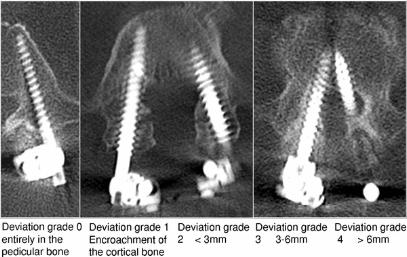
\includegraphics[width=0.5\textwidth]{assets/deviation.jpg}
	\caption{Grading of pedicle screw placement errors}
	\label{fig:dev}
\end{figure}


Conventionally, the process for inserting pedicle screws was as follows:
First, a large insicion would be made in the patients back, near
where the screws will be placed. Then the surgeon uses an bone awl tool
to puncture a hole in the outside layer of the bone, before working the
sharp tip of the tool through the soft inner part of the bone. The surgeon
relies on previous experience of the resistance of different types of bone to
determine the correct heading for the tool. Once the hole has been created,
the pedicle screw is inserted\cite{Manbachi2016}.

With the advent of technology, this method has been augmented with the use of computers to
create a process known as image-guided surgery (IGS)\cite{Azad2016}. An example of IGS is shown in Figure \ref{fig:igs}.
These techniques allow
visualisation of the location of operation through the use of visual markers that are
placed on the patient and surgical tools. The markers are tracked by optical positioning sensors. Utilising this
information in reference to computed tomography (CT) scan taken before surgery enables surgeons to limit the
probability of complications through greater awareness of the topology of the operational environment\cite{Costa2011}.

\begin{figure}[h!]
	\centering
	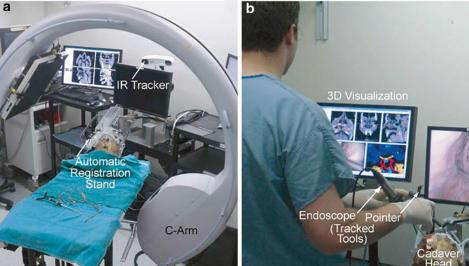
\includegraphics[width=0.5\textwidth]{assets/igs}
	\caption{Optical tracking system utilising several cameras to track locations of infrared markers\cite{Manbachi2016}}
	\label{fig:igs}
\end{figure}


T. Laine et al conducted a study on 100 patients using the tradidional method and the 
computer assisted method, and found that IGS reduced the pedicle wall perforation rates by 
nearly a quarter across all screws inserted, as shown in Table \ref{tab:accuracy}\cite{Laine2000}.
\begin{table}[h!]
	\centering
	\begin{tabular}{l l l l }
		& \shortstack{Conventional\\screw insertion} & \shortstack{Computer-assisted\\insertion} & Total \\ \hline
		Medial & 21 & 1 & 22 \\ \hline
		Inferior & 7 & 0 & 7 \\ \hline
		Lateral & 9 & 9 & 18 \\ \hline
		Superior & 0 & 0 & 0 \\ \hline
		Total & 37 &10 & 47 \\
	\end{tabular}
	\caption{Number of pedicle perforations in different locations\cite{Laine2000}}
	\label{tab:accuracy}
\end{table}

The use of IGS does appear to reduce the risks involved with spinal surgery, 
however, this method does have limitations. Due to the use of optical technologies for the object tracking, the
system is limited to line of sight, which means that the surgical team must remain out of the way of the locating
equipment. 

Furthermore, considerable force is used in the implantation of the pedicle screws, and this force can
result in bending deformations in both the screws and equipment\cite{Chatzistergos2010}. As these deformations occur without
affecting the position of the visual markers, errors can occur in the ability for the system to precisely locate the
position of the pedicle screws\cite{Castro1996}.


A potential solution to these inherent issues involves the use of several sensing methods to avoid the errors
currently encountered. In order to account for bending moments within the equipment and screw, silver
nanowire based strain sensors will be utilised to track bending deformations in multiple dimensions. To provide
real time-visualisation of objects and structures within the body, a tool with short-wavelength ultrasonic sensors will
replace currently used tools. In order to make full use of the feedback from these sensors, robotic guidance
systems will be employed to assist surgeons in correctly implanting the pedicle screws. 

It is hoped these changes to the current workflow will
overcome limitations in current methodology and therefore improve patient outcomes by reducing pedicle screw
misplacement. This paper will present a proposal for the above methods and their possible contribution to the field
of spinal surgery, based on information available in online peer-reviewed papers.


\section{Silver Nanowire Strain Sensors}


In order to maintain accurate information on the position of the tip of the pedicle screw relative to the
implanting tool, any deformation of the tool and/or screw must be measured. These deformations result from the
forces involved in the implantation of the screw, both those induced by the driving mechanism and by the
reaction forces of the bone on the screw. The design of medical pedicle screws does include a small hollow
section into which a sensor might be included, but the small size of the screw implies a very small sensor. A
possible solution is the use of nanowire/polymer sensors to measure strain induced by bending of the instrument
or screw.

Silver nanowire sensors are composed of thin networks of silver alloys (Ag NWs) implanted just beneath the
surface of polymer substrates\cite{Amjadi2014}\cite{Lee2016}. These configurations exhibit high conductivity and due to their composite
nature show resistance to instability that have characterised previous Ag NW based sensors\cite{Lee2016}. The sensitivity
of the strain gauge can also be selectively engineered by varying the surface coverage and waviness of the
nanowire networks\cite{Xu2012}.

\begin{figure}[h!]
	\centering
	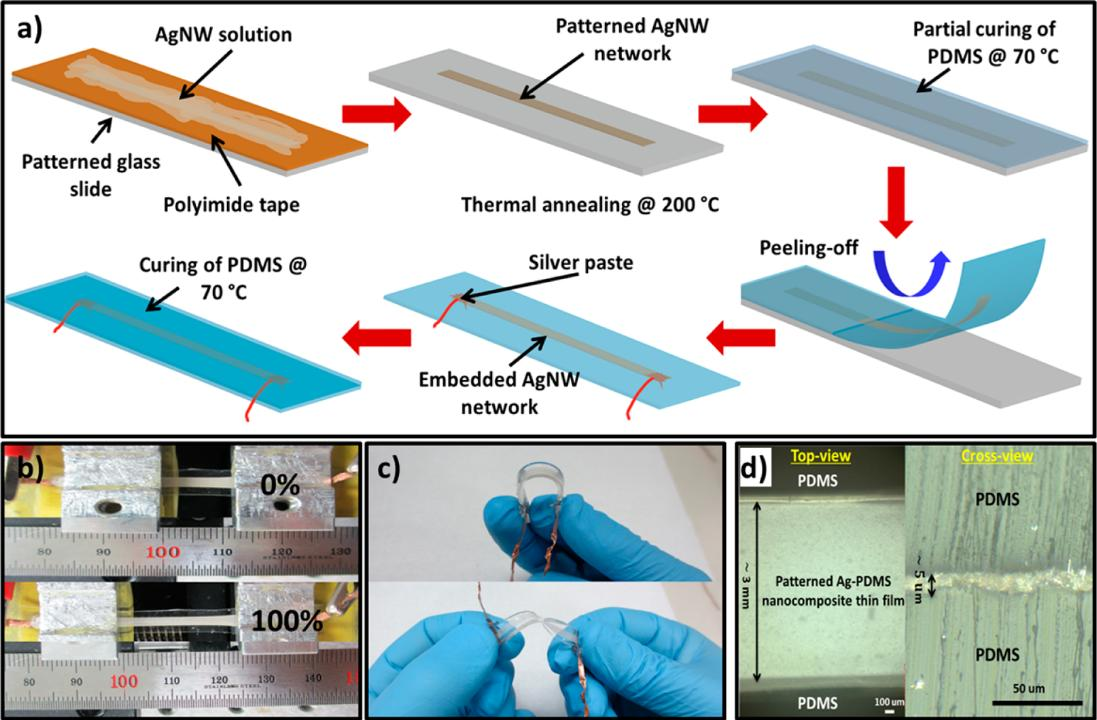
\includegraphics[width=0.5\textwidth]{assets/manufacturingNano.jpg}
	\caption{Manufacturing of AgNW structures on PDMS substrates\cite{Amjadi2014}}
	\label{fig:manufacture}
\end{figure}

Ag NWs can be configured to measure strain through a change in the capacitance of the system\cite{Ho2015} or through
changes in the resistance of the wires due to the imposed strain.



An obvious drawback of this system is that it does not account for bending moments, but rather axial strain.
However, if multiple such sensors are assembled into an array such that each is arranged around a central core
such that the substrate fibres are equally distributed around the core, then the moment imposed on the system
can be calculated by comparison of the axial loads induced in the various sensors. In order that bending can be
determined in two axes, two opposed pairs of sensors would be laid orthogonally to one another along the
substrate rods, as shown in Figure \ref{fig:potential}. An array of nanowire sensors was
found to be able to accurately record tip deflections of less than a millimetre in magnitude, which implies that it
is suitable for this application.\cite{Ho2015}

\begin{figure}[h!]
	\centering
	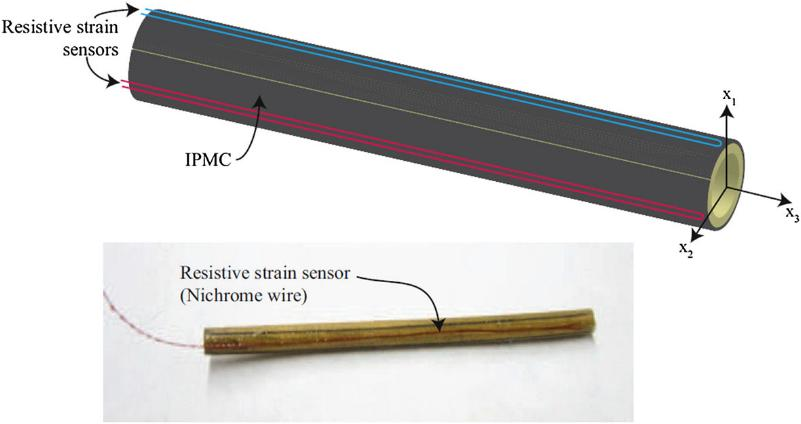
\includegraphics[width=0.5\textwidth]{assets/sensorSetup.jpg}
	\caption{Potential sensor setup with multiple axis sensing\cite{Tsugawa2015}}
	\label{fig:potential}
\end{figure}

\begin{figure}[h!]
	\centering
	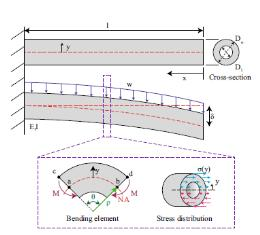
\includegraphics{assets/bendingDeformation.jpg}
	\caption{Diagrammatic representation of sensor tube undergoing bending deformation\cite{Tsugawa2015}}
	\label{fig:deviation}
\end{figure}

In order to measure bending forces in this manner, the ends of the fibres must be fixed such that strain induced
is in the axial direction. Therefore, the sensors and supporting core would be clad in a protective housing,
composed of medical grade stainless steel. Two options would exist for implementation. Firstly, a single
housing would run the length of the tool and extend out such that it could be inserted directly into the screw and
thus measure the bending of the overall system. Secondly, two such housings would be used, one for the tool
and a shorter one to measure the bending in the screw. We would likely employ the two-cylinder approach as it
would avoid undue shear stresses acting on the sensor housing if the tool slipped during operation.


\section{Ultrasonic Image Guidance}
Ultrasound is an imaging technique that involves emmiting sound waves into a
body. The sound waves are above the limit of human hearing, often being in
the order of mHz. An image is created by capturing the waves reflected
by the organs in the body. 
The process relies on the fact that the sound will interact with
different areas of the body differently depending on their density and
structure\cite{ultraHist}. A common use for ultrasonic imaging is obstetric ultrasound,
the process of examining the wombs of pregnant women. 

Ultrasound has several advantages over other types of imaging, including:
being non-invasive, safe and relatively painless, not using ionising radiation,
not requiring an injection of a contrast medium and being able to be used in
many different areas of the body\cite{imagingExplained}. 

Bone is a rigid organ that developed to, among other things, 
provide structural support for the human body. It is made primarily of
collagen, is has two different macro level structures: Cortical and Canellous 
bone. The cortical bone makes up the exterior of the bone, and is a hard, 
densely packed structure. Canellous bone, on the other hand, makes up the
interior of the bone, and appears porous and sponge like. These structures
can be seen in Figure \ref{fig:boneStruct}.

\begin{figure}
	\centering
	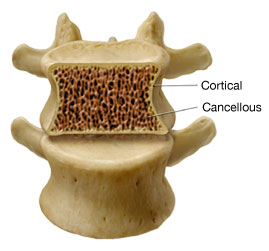
\includegraphics{assets/boneStruct.jpg}
	\caption{Cortical and Cancellous bone structures \cite{boneStructure}}
	\label{fig:boneStruct}
\end{figure}

Differences between the structures of the 2 different components of bones
provide a way with which the accuracy of the placement of a pedicle screw hole
can be measured in real time. The proposed method is to use an ultrasonic 
sensor to determine the differences in density between the two bone structures
in the hope that the accuracy of the hole trajectory can be determined by the
surgeon in real time without line of sight on the operating area. 

The sensor will be an array of ultrasonic transducers embedded into the awl
tool used for making the hole for the pedicle screw. The general working
concept of this sensor can be seen in Figure \ref{fig:ultraArray}.
In frame A of \ref{fig:ultraArray}, the sensor array is pictured approaching
the bone. In frame B, the trajectory is on a collision course with the wall 
of the bone, and will cause a pedicle perforation if not corrected. This
is demonstrated by the red section of the ultrasound image, demonstrating 
the higher density of the cortical bone. Finally, frame C shows a well placed
trajectory.


This method has a number
of benefits, including: integration into the current pedicle screw insertion
workflow, no emmision of ionising radiation, as well as being able to determine
the trajectory of the awl in real time.

\begin{figure}[h!]
	\centering
	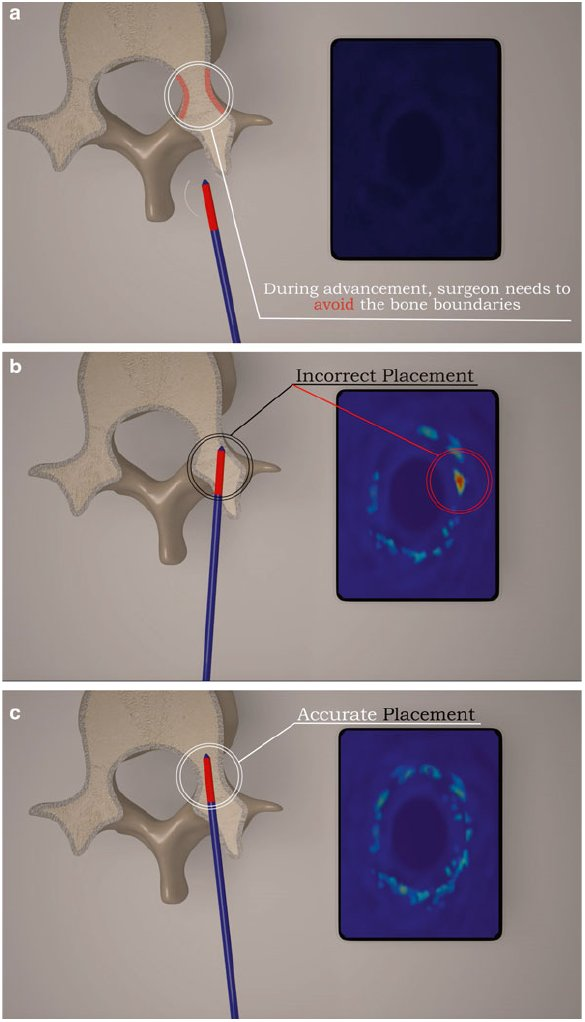
\includegraphics[width=0.5\textwidth]{assets/ultraArray.jpg}
	\caption{Demonstration of the concept of an awl tool with integrated ultrasonic sensor array\cite{Manbachi2016}}
	\label{fig:ultraArray}
\end{figure}

Using an ultrasonic sensor in bone presents some difficulties, as bone attenuates
the signal quickly. Traditional ultrasound devices used for imaging soft
human tissue normally operate in the region of 19-20MHz. At this frequency,
the attenuation reduces the penetration of the sound to unusable levels\cite{Laugier2011}.
To increase the penetration of the signal, the frequency of sound must be reduced, however,
when the frequency is reduced the resolution of the ultrasoung is also reduced. In 2008 Mujagić
et al found that decreasing the bandwidth of the ultrasound down to 1-3.5MHz allowed them to
correctly detect an aluminium reflector through bone specimens ranging from 1-1.9cm in thickness in
83.2$\%$ of cases at 1MHz and 70.1$\%$ of cases at 3.5MHz. Furthermore, the boundaries
of the specimens we idetifiable ``with clinically sufficient average accuracy of 1.1mm and 0.9mm in the 1MHz
and 3.5MHz'' images, respectively\cite{Mujagic2008}. This would indicate that the 
problems presented by the bone attenuating the signal can be avoided without too much
difficulty.



\section{Robotic Surgical Equipment}
Due to the requirement for extremely precise insertion of tools, robotic apparatus have been
developed for use in spinal surgeries. Devices guide the surgeon towards an insertion trajectory
determined pre-operation\cite{Hu2012}. The utilisation of these systems in conjunction with pre-operative
imaging has produced improved patient outcomes, with an accuracy of less than 2mm being
achieved 94.5$\%$ of the time as compared to 91.5$\%$ of the time for unassisted surgeries\cite{Kantelhardt2011}.
Furthermore, the use of robotic assistance can allow the use of less initial imaging, with benefits
to the patient from lower radiation doses.

One possible difficulty that may be encountered when designing a robot for performing
spine surgery might be the need to quantify the accuracy of the tools used. As mentioned
previously, the bending of tools can be a source of error that would not show up on the
current robotic systems. As a solution to this, the proposed nanowire sensors could
be fed directly into the robot, which can then compensate for that error, rather than 
simply display the information for a human to interpret.

In addition to this, the real-time feedback from the ultrasonic sensors could warn surgeons
if the planned path was unexpectedly in danger of screw misplacement. Alternatively, the 
data taken from the ultrasonic sensor arracy could be sent directly to the robot, which
would then change its trajectory appropriately.


\section{Conclusion}
The rapid expansion of the scope of technology in the world today has
lead to improvements in the accuracy and repeatability of pedicle screw insertion
operations. Computer assisted surgery can decrease the pedicle perforation rate
by up to 75$\%$ in some cases\cite{Laine2000}. Despite this, there are still some
challenges that face the current technology, namely the inability to detect tool
bending during IGS operation, and the requirement of line of site for the sensors
which can reduce operating space of the surgeon. The tool bending problem can be
remedied by embedding nanowire strain sensors into the tools to detect bending.
The line of sight problem can be solved by using an awl with an ultrasonic
array built into the end to detect the bone wall. Both of these solutions 
should provide increased accuracy of pedicle screw placement, and could be
further enhanced by removing the surgeon from the surgery entirely and
making a robot to perform the surgery with these enhanced sensors.




% trigger a \newpage just before the given reference
% number - used to balance the columns on the last page
% adjust value as needed - may need to be readjusted if
% the document is modified later
%\IEEEtriggeratref{8}
% The "triggered" command can be changed if desired:
%\IEEEtriggercmd{\enlargethispage{-5in}}

% references section

%\bibliographystyle{IEEEtran.bst}
%\bibliography{IEEEabrv,../bib/paper}

\bibliography{report}
\bibliographystyle{IEEEtran}

% insert where needed to balance the two columns on the last page
%\newpage


\end{document}



